
%todo:
%-try an S2 model of prevalence judgement task, too. does it reduce to the L1 model?
%- figure out which plots to use for fixed-threshold and lvRSA  (both TFBT stuff and posterior predictives)
% - do we really want posterior predictives that include the guessing parameter? (the guessing parameter is part of the analysis model, not the cognitive model...)
%- what kind of evidence do we want to use at the end to relate inferred priors to elicited? 
%	- is eye-balling the elicited prior and the mean inferred priors sufficient?
%	- i tried TFBT on the elicited priors to back out gamma & deltas, but gammas don't seem to come apart for DD vs. plain (as they do in the inferred priors from Exp 1 &2)
%	- one possible way to get this sort of "ordered gammas" evidence would be to repeat the prior elicitation with more items per trial
%		- the thought is that in our prior elicitation, i used 5 animals per slide (and 6 trials)
%			- probably there was not enough dynamic range for Plain vs DD to come apart 
%		- i think with 10 items, it would be better (but does that mean just 3 trials, one in each context, per subj?) [there are only 30 animals]
%		
%todo after cogsci:
%-run additional contexts. e.g. separate dangerous and distinct.
%-look again at finer-grained truth judgement task?
%-think about the weird cases of generics in the literature. e.g. ``robins lay eggs''.
%




\documentclass[10pt,letterpaper]{article}

\usepackage{cogsci}
\usepackage{pslatex}
\usepackage{apacite}
\usepackage{url}
\usepackage{graphicx}
\usepackage{caption}
\usepackage{subcaption}
\usepackage{listings}
\usepackage{color}
\usepackage{textcomp}
\usepackage{amsmath}
\usepackage{amssymb}

\graphicspath{{figures/}}

\def\signed #1{{\leavevmode\unskip\nobreak\hfil\penalty50\hskip2em
  \hbox{}\nobreak\hfil(#1)%
  \parfillskip=0pt \finalhyphendemerits=0 \endgraf}}

\newsavebox\mybox
\newenvironment{aquote}[1]
  {\savebox\mybox{#1}\begin{quote}}
  {\signed{\usebox\mybox}\end{quote}}


\lstset{
  language=Scheme, % Andreas Stuhlmuller. Scheme listings. https://github.com/stuhlmueller/scheme-listings.git
  columns=fixed,
  tabsize=2,
  extendedchars=true,
  breaklines=true,
  frame=single,
%  numbers=left,
  numbersep=5pt,
   basicstyle=\scriptsize\ttfamily
%  rulesepcolor=\color{solarized@base03},
%  numberstyle=\tiny\color{solarized@base01},
%  keywordstyle=\color{solarized@green},
%  stringstyle=\color{solarized@cyan}\ttfamily,
%  identifierstyle=\color{blue},
%  commentstyle=\color{solarized@base01},
%  emphstyle=\color{solarized@red}
}

\definecolor{Red}{RGB}{255,0,0}
\newcommand{\red}[1]{\textcolor{Red}{#1}}  


\title{Generics are vague: formalizing the scalar semantics of generic language}
 
 \author{{\large \bf Michael Henry Tessler, Noah D. Goodman } \\
	\{mhtessler, ngoodman\}@stanford.edu \\
  Department of Psychology, Stanford University}
 
\begin{document}
\maketitle


\begin{abstract}
Insert abstract here.

\textbf{Keywords:} 
generics; pragmatics; bayesian cognition; bayesian data analysis
\end{abstract}

\begin{aquote}{Barack Obama, \emph{2015 State of the Union Address}}
New sanctions passed by this Congress, at this moment in time, will all but guarantee that diplomacy fails -- alienating America from its allies; making it harder to maintain sanctions; and ensuring that Iran starts up its nuclear program again.
\end{aquote}


Generic meanings are hard to pin down.  Consider President Obama's remark during the State of the Union Address. The sentence is a generic statement about \emph{new sanctions} in that it conveys a generalization about the members of a kind \cite{Carlson1977, Leslie2008}. It invites the question: ``Exactly how many of these new sanctions will guarantee diplomacy fails?'' President Obama's statement is conceivably true if most or only a few new sanctions will be problematic. At the same time, he is not a man to waste words---why does he go through the trouble of saying such a vague statement? In this paper, we will see that both the context in which his words are uttered and his effort in producing this statement contribute to the meaning we derive. We will propose that these aspects of generic statements follow from pragmatic reasoning about an uncertain threshold for meaning; an idea which we formalize in a Bayesian Rational Speech Acts computational model.

Generic statements are puzzling because their meaning is so flexible. On one hand, generics would seem to suggest an almost universal quantification, as in ``Dogs bark''. Others, like ``Mosquitos carry West Nile virus'', involve a property that applies only to a small subset of the kind. 
%It is perhaps this inherent uncertainty that leads generics to be so widespread in natural language. 
\citeA{Cimpian2010} (henceforth, CBG) carried out a series of controlled studies designed to examine the truth conditions and implications of generic statements. 
They found evidence for the influence of context, in the form of additional knowledge about a target property, on participants' willingness to accept generic statements (i.e. context modified the truth conditions). CBG also found an asymmetry between verification and interpretation: participants interpreted a generic (e.g.~``lorches have purple fur'') as nearly universal, but would endorse the same generic as true if given a much lower prevalence level (``50\% of lorches have purple fur'').

Both context and asymmetry effects pose a puzzle for formal semantics. 
In this paper, we seek to explain both of these phenomena as the effects of pragmatic inference filling in a meaning that is underspecified in the semantics. 
In particular, we posit a scalar semantics for generics in which they express that prevalence---the probability of the property given the kind---is above a threshold (Cf. \cite{cohen}). Following \citeA{lassiter} we treat this threshold as a free variable that is reasoned about by a pragmatic listener: what is the threshold likely to be, given that a speaker bothered to utter the generic? Context effects follow from differences in prior beliefs about the distribution of the property across categories. Asymmetry effects follow directly by modeling differences in the language understanding and production task faced by participants in the different experiments (Cf. \citeA{Degen2014}).  %suggested that different dependent measures in experimental pragmatics paradigms map onto different communicative roles, and thus should be modeled accordingly. 

%We draw on new advances in probabilistic pragmatics to formalize two possible theories of the generic. Further, we harness the power of Bayesian data analysis to mediate between these formal theories and draw inferences about cognitively interesting model parameters. 

In what follows, we first replicate the main effects reported by CBG, using Bayesian data analysis techniques to further examine the effective truth-conditions of generic statements. We then introduce a model of generic comprehension, within the probabilistic Rational Speech Acts framework \cite{Frank2012,Goodman2013}. We show that this model predicts both context and asymmetry effects, given appropriate prevalence priors. Finally we experimentally elicit the prevalence priors in CBG's experimental contexts, verifying the predictions of the model.


%(e.g. ``These feathers are as sharp as needles and can easily get lodged in you, causing massive bleeding. No other animals have these kinds of feathers'')
% (e.g.  ``These feathers are wide and very smooth to the touch. Other animals have these kinds of feathers.'')

%How are we to understand these data? One interpretation is that context changes the truth-conditions for a generic statement, but that within a context, the truth-conditions are stable. A different sort of explanation is that context changes the nature of world somehow, and that generic meanings are inferred rationally from context. We draw on recent advances in probabilistic pragmatics and Bayesian data analysis to mediate between these two alternatives.


\section{Experiment 1: CBG replication}

In CBG's \emph{truth conditions} task, participants were given an evidence statement consisting of the percentage of a category that had a property (e.g. ``30\% of lorches have purple feathers.''). Participants were asked whether the associated generic statement (i.e. ``Lorches have purple feathers'') was true or false. The authors manipulated context within-subjects by adding additional statements about the property. Three contexts we will focus on in this paper are \emph{dangerous and distinct} (DD, e.g.~``These feathers are as sharp as needles and can easily get lodged in you, causing massive bleeding. No other animals have these kinds of feathers''), \emph{not distinct and irrelevant} (NI, e.g.~``These feathers are wide and very smooth to the touch. Other animals have these kinds of feathers.''), and \emph{plain} (P, no additional statements). The authors found that DD increased the overall proportion of ``true'' responses of the generic propositions. 
%That is, when the property in question was dangerous and distinct, participants required a lower overall prevalence (e.g. 10\% of lorches had purple feathers) to assert that the generic statement was true.
In their \emph{implied prevalence} task, participants were supplied with the generic (again with context as a within-subjects variable) and asked to judge prevalence: ``What percentage of lorches do you think have purple feathers?''. The authors consistently found that the generic was interpreted strongly---nearly all lorches have purple feathers. 

Experiment 1 attempted to replicate the main findings of CBG: that context affects the proportion of ``true'' responses to a generic statement (Exp. 1a) and that there is an asymmetry between interpretation and verification of the truth conditions of the generic (Exp. 1b). 
Exp. 1a and 1b were conducted on separate sessions, one week apart. None of the participants completed both experiments.

\subsection{Experiment 1a: \emph{truth conditions}}

\subsubsection{Participants}

We recruited 40 participants over Amazon's crowd-sourcing platform Mechanical Turk.  
%NDG: restrictions on IP address or native language?

\subsubsection{Procedure and materials}

Our procedure was very similar to CBG \emph{truth conditions} task. Our instructions were elaborated to improve interest and motivation\footnote{The experiment in full can be viewed at \url{http://stanford.edu/~mtessler/experiments/generics/cbg2010-replication/experiment/experiment-9.html}}. 

We used the same materials as CBG (available in their Appendix). The materials used were 30 novel animals (e.g. lorches, morseths, blins) each paired with a unique property. Properties were pairs of colors and body-parts (e.g. purple feathers, orange tails). Each participant saw 30 unique animal-property pairs: 10 in each of 3 contexts \{\emph{plain}, \emph{DD}, \emph{NI}\}. The 10 items in each context were randomly paired with 1 of 5 ``prevalence levels'': \{10, 30, 50, 70, 90\}\%; each prevalence level appeared 2 times per context. 

Participants saw a prevalence statement and a context statement (\emph{plain}, \emph{DD}, \emph{NI}, as illustrated above). 
%A context here was either (1) dangerous \& distinct statements (e.g. ``These feathers are as sharp as needles and can easily get lodged in you, causing massive bleeding. No other animals have these kinds of feathers.''), (2) not distinct \& irrelevant statements (e.g. ``These feathers are wide and very smooth to the touch. Other animals have these kinds of feathers.'', or (3) nothing else. 
Participants were then asked ``Is the following sentence true or false?'', below which was presented the associated generic (e.g. ``Lorches have purple feathers'') and 2 radio buttons. 

\subsubsection{Results}


\begin{figure}
        \centering
        \begin{subfigure}[b]{0.55\columnwidth}
                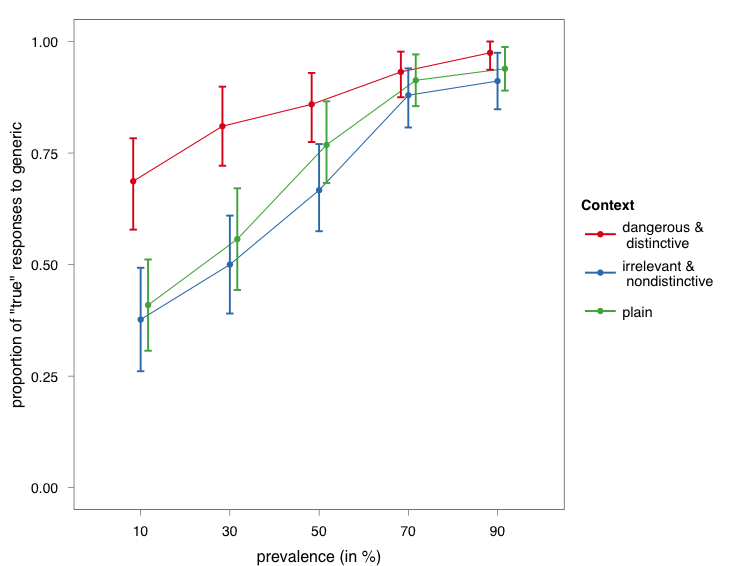
\includegraphics[width=\columnwidth]{data_truthconditions1}
                \caption{Truth conditions of the generic vary across contexts}
                \label{fig:datatc}
        \end{subfigure}%
        ~ %add desired spacing between images, e. g. ~, \quad, \qquad, \hfill etc.
          %(or a blank line to force the subfigure onto a new line)
        \begin{subfigure}[b]{0.45\columnwidth}
                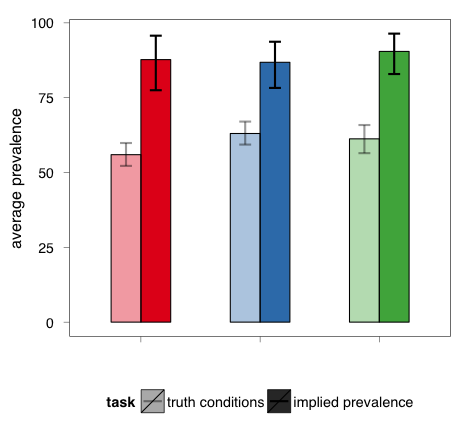
\includegraphics[width=\columnwidth]{data_asymmetry1}
                \caption{Asymmetry between verification and interpretation}
                \label{fig:datasym}
        \end{subfigure}
        ~ %add desired spacing between images, e. g. ~, \quad, \qquad, \hfill etc.
          %(or a blank line to force the subfigure onto a new line)
        \caption{Replication of CBG}\label{fig:exp1}
\end{figure}



%\begin{figure}
%\centering
%    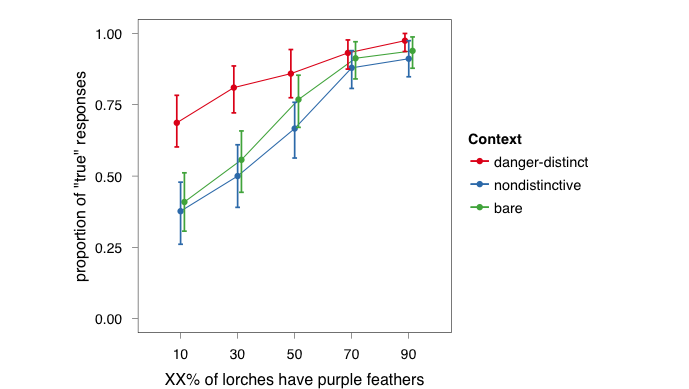
\includegraphics[width=\columnwidth]{fig1_replication}
%    \caption{Replication of CBG \emph{truth conditions}, generics condition}
%  \label{fig:replication}
%\end{figure}


Our results replicated the finding of CBG that the generic statement was endorsed more in the dangerous and distinctive context than in the other two contexts (Figure \ref{fig:datatc})\red{[insert stats here]}. There was also an interaction between prevalence level and context such that the DD context was endorsed more at lower prevalence levels. \red{[insert stats here]}. 

\subsection{Experiment 1b: \emph{implied prevalence}}

\subsubsection{Participants}

We recruited 30 participants over Amazon's crowd-sourcing platform Mechanical Turk.  

\subsubsection{Procedure and materials}

Our procedure was very similar to CBG \emph{implied prevalence} task. Our instructions were elaborated to improve interest and motivation\footnote{The experiment in full can be viewed at \url{http://stanford.edu/~mtessler/experiments/generics/cbg2010-replication/experiment/experiment-12.html}}. 

The materials and context conditions were the same as in Exp. 1a. 
On each trial, participants saw a generic statement (instead of a prevalence statement) and a context. 
%A context here was either (1) dangerous \& distinct statements (e.g. ``These feathers are as sharp as needles and can easily get lodged in you, causing massive bleeding. No other animals have these kinds of feathers.''), (2) not distinct \& irrelevant statements (e.g. ``These feathers are wide and very smooth to the touch. Other animals have these kinds of feathers.'', or (3) nothing else. 
Participants were then asked ``What percentage of \emph{the kind} do you think have \emph{the property?}'' (e.g. ``What percentage of lorches do you think have  purple feathers?''). The dependent measure was a free response required to be an integer, $0-100$. 

\subsubsection{Data analysis and results}

%\begin{figure}
%\centering
%    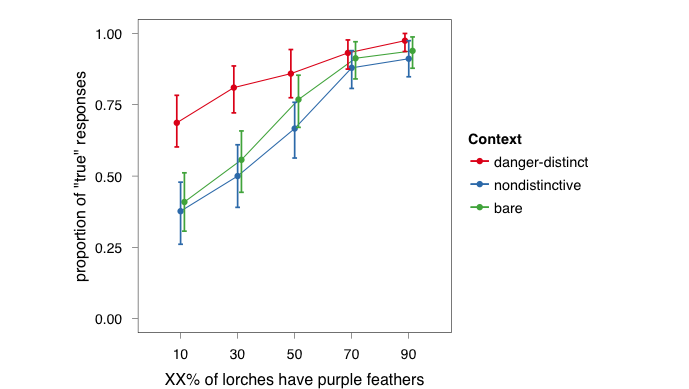
\includegraphics[width=\columnwidth]{fig1_replication}
%    \caption{Replication of CBG \emph{asymmetry}, generics condition}
%  \label{fig:replication}
%\end{figure}
%

Our results replicated the finding of CBG that the generic statement was interpreted as having a higher prevalence than its truth conditions would imply. 
\red{say something about how this analysis was done...}

\section{Fixed-threshold semantics}
The above results, replicated from CBG, indirectly constrain the truth conditions that participants are effectively using for generic statements within these experimental conditions. In this section we explore these truth conditions more directly by using bayesian data analysis techniques.
We assume that the conditions for truth of the generic can be usefully represented by a threshold on prevalence: the generic is true when the prevalence of some property within a kind exceeds a given threshold (See \cite{cohen} for a similar assumption).


\subsection{A truly fixed semantics}
We first examine what this threshold would look like, if it were a truly fixed-threshold. 


\[
 g(x) =
  \begin{cases}
   1 & \text{if } x > \theta \\
   0       & \text{if } x \leq \theta
  \end{cases}
\]

Here, x is some proportion of a kind with a property. We can then ask, how must the threshold be set to account for the data observed? We assume a uniform prior distribution over possible values of $\theta$. Following standard practice in Bayesian data analysis \cite{LW2014}, we include the data-analytic parameter $\phi$ to account for data points that deviate strongly from our theory; it is a guessing parameter. We assume there is some proportion of responses\footnote{Ideally, we would have $\phi$ be a function of participant (some participants guess more than others) and experimental condition (some conditions are more difficult or less constrained and invite more guessing). As a first pass, we assume there is some global quantity of guessing.} where the participant is responding randomly, and we estimate this quantity by way of $\phi$.

\begin{align}
\theta_{generic} \thicksim U(0,1) \\
\phi_{t} \thicksim U(0,1) %\mid  t \in \{exp1a, exp1b\}
\end{align}
%We formalize the notion of ``effective truth conditions'' by saying the generic is a function from states of the world to truth-values. We operationalize \emph{states of the world} here as the prevalence of some property within a kind. This mapping is then determined by some threshold such that the generic is true when the prevalence is above threshold. 

%Using the Church probabilistic programming language to represent this model \cite{probmods}, this would be written:
%
%\begin{lstlisting}
%(define generic 
%	(lambda (prevalence) (> prevalence generic-threshold)))
%\end{lstlisting}

%To handle the inference problem the participant is faced with, we express the subject's uncertainty about whether the generic is true or false.
%
%\red{NDG: the rest of this section is too long and doesn't make sense to me...}
% \begin{lstlisting}
%(define truth-conditions (lambda (prevalence)
%	(query  
%	
%		(define generic ...) ;defined as above
%		(define generic-is-true? (flip 0.5))
%		
%		generic-is-true?
%			
%		(generic prevalence))))
%\end{lstlisting}

\subsubsection{Results}

The results are shown in Figure \ref{fig:totallyfixed}. 


From this model, we get the idea that the generic could be true for anywhere between 10\% and 30\%, but this can account for no data that would vary by context.

\subsection{A relaxed but fixed semantics}

 In Exp. 1a, we found evidence that the generic truth conditions did vary by context. Thus, we reexamine our fixed-semantics model, now allowing for the possibility that $\theta$ could vary by context.


\[
 g(x, c) =
  \begin{cases}
   1 & \text{if } x > \theta_{c} \\
   0       & \text{if } x \leq \theta_{c}
  \end{cases}
\]

Again, we put uniform priors over each of the $\theta_{c}$'s. We are now in a position to ask how the truth-functional threshold of the generic behaves across these three contexts. 

\subsubsection{Results}

The results can be seen in Figure \ref{fig:bda1a}. In the \emph{plain} condition, the analysis suggests the threshold is somewhere between 0\% and 30\%, but it's unclear where exactly in that range the threshold should be\footnote{This uncertainty results from the sparseness of our sampling (see Procedures and Materials). Participants were queried only at prevalence levels 10, 30, 50, 70, and 90}. Critically, in the \emph{dangerous and distinctive} context, the analysis infers a lower threshold, less than 10\%. This matches with intuition and the empirical results, that a dangerous and distinctive context allows for the generic to be more permissive (e.g. ``Mosquitos carry West Nile Virus'' is true, even though very few mosquitoes actually do). Finally, and most intriguingly, the analysis infers a third distinct threshold profile for the \emph{nondistinct and irrelevant} context.  For this, it says that threshold is greater than 10\%, but could be as high as 50\%. This is an overall higher inferred threshold for the nondistinctive category and an aspect of analysis totally obscured by standard frequentist estimation. 

This model is too a simple model, however. We see this in part by the posterior distribution of the data analysis parameter \lstinline{phi}. This parameter is one measure of fit because it represents the percentage of responses that the data analysis model wants to attribute to guessing. With this cognitive model, the percentage of guesses is somewhere between 40\% and 50\%. The amount of guessing is so high because our computational model is inflexible.



%A \lstinline{query} is a special function in Church. The first arguments to a query function are a generative model: definitions or the background knowledge with which a reasoning agent is endowed. Definitions for which a random choice is stipulated (e.g. \lstinline{(define generic-is-true? (flip 0.5))}) denote aspects of the world over which the agent has uncertainty. The second argument, called the \emph{query expression}, is the aspect of the computation that the model should return. The final argument, called the \emph{conditioner}, is the information with which the agent updates beliefs. 
%
%This is the simplest model of the truth conditions of the generic. It says the subject has maximal uncertainty as to whether or not the generic is true (expressed by \lstinline{(flip 0.5)}, a Bernoulli random variable). The subject uses the prevalence given to her to determine if the generic is true. 
%
%At the same time, we want to take into account the results of Exp. 1b: the interpretation of the generic. Here, we are concerned with the interpretation of the utterance, so we put uncertainty over the prevalence. We condition on the fact that the generic must be true of the prevalence, whatever it may turn out to be.
%
% \begin{lstlisting}
%(define implied-prevalence (lambda (utterance)
%	(query  
%		
%		(define generic ...) ;defined as above
%		(define prevalence (uniform 0 1))
%		
%		prevalence
%			
%		(generic prevalence))))
%\end{lstlisting}
%
%We are now in a position to ask how the truth-functional threshold of the generic behaves across these three contexts. To do this, put each of these models inside of a Bayesian data analysis model. The data analysis model posits that \lstinline{generic-threshold} might be a function of context.
%
%The data analysis model can be written very simply in Church.
%
%\begin{lstlisting}
%(define bayesian-data-analysis 
%	(query
%		; we don't know the generic threshold but we feel it might be a function of context
%		(define generic-threshold 
%			(mem (lambda (context) (uniform 0 1))))
%		(define truth-conditions ...) ; defined as above
%		(define implied-prevalence ...)
%		
%		(define phi (uniform 0 1)); guessing parameter
%				
%		generic-threshold ; return generic-threshold	
%		
%		(and 
%			(= experiment1a-data truth-conditions)
%			(= experiment1b-data implied-prevalence))))
%
%\end{lstlisting}
%
%The model above is a data analysis model to try to infer the threshold of the generic, with the built-in flexibility that it might vary by context. The functions \lstinline{truth-conditions} and \lstinline{implied-prevalence} jointly form our cognitive theory\footnote{This could be made more explicit by moving the function \lstinline{generic} outside of either \lstinline{query}, since it is the same function. This function is the core of this cognitive theory.}. It says the generic is like an alien quantifier. This quantifier behaves like other quantifiers in that it has a fixed-threshold semantics. The only thing special about the generic is that the threshold might be different for different contexts. 
%
%We don't know what the generic might mean \emph{a priori}. Thus, the generic-threshold\footnote{If the generic threshold turns out to be 0, the generic ``Lorches have purple feathers'' would mean essentially, ``Some lorches have purple feathers''. If the threshold turned out to be very close to 1, the generic would mean essentially: ``All lorches have purple feathers''.} follows a uniform prior distribution between 0 and 1. 
%
%The \lstinline{query} function is written to return \lstinline{generic-threshold}, which is the parameter we are interested in inferring. Finally, the last line is our condition statement: we condition on the data we collected in Exp. 1a being explained by the \lstinline{truth-conditions} model and Exp. 1b to be explained by \lstinline{implied-prevalence}. For clarity, we have omitted the impact of \lstinline{phi}, but it comes into play in the condition statement. In reality, each response could have been generated by our theory (via \lstinline{truth-conditions} or \lstinline{implied-prevalence}) or by guessing (via \lstinline{phi}).  

\subsection{Results}

\subsubsection{Inferred parameters}

\begin{figure}
\centering
    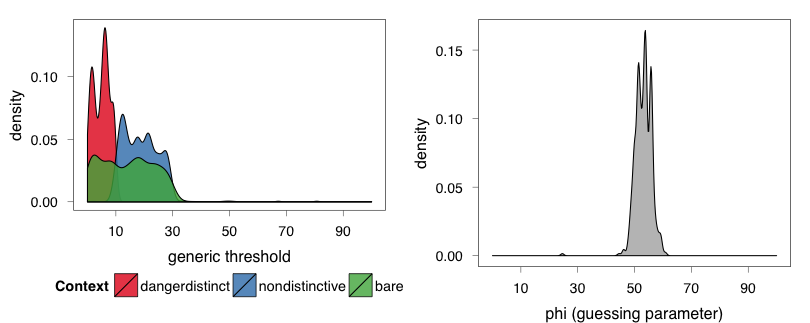
\includegraphics[width=\columnwidth]{fig2_bda1_combined}
    \caption{Inferred threshold for the generic across contexts}
  \label{fig:bda1a}
\end{figure}


\subsubsection{Posterior predictives}

This can also be seen in the posterior predictive distribution of responses (Figure \ref{fig:bda1posteriorpred}, left). 

The posterior predictive distribution marginalizes over the inferred parameter values to produce predictions about what the data should look like given the cognitive model and the inferred data. This is an important step in model validation as it shows what the model actually predicts the data should look like \footnote{As a thought experiment, consider 2 coins assumed to come from a single coin-making machine (all the coins of this machine have the same weight). You flip each 100 times. The first one returns 100 heads, and the second one returns 100 tails. The posterior mean of the inferred coin weight will be 0.5. Comparing the posterior predictive distribution (based on this inferred coin-weight) to the observed data will highlight the fact that your theory about the ``single coin-making machine'' is seriously flawed.}.

The model matches the ordering of the truth-conditions by context reasonably well, but is too dichotomous in its predictions. The correlation between the posterior predictive and the data is $r = 0.81$. 

\begin{figure}
\centering
    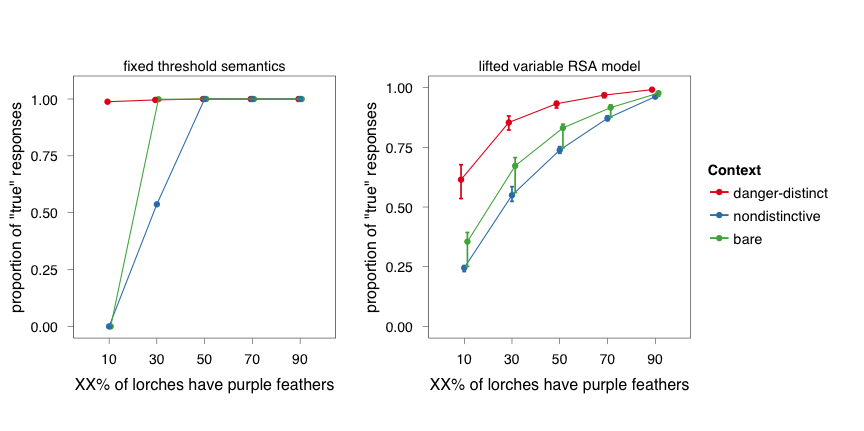
\includegraphics[width=\columnwidth]{fig3_2pps}
    \caption{Posterior predictive using fixed-threshold semantics (left) and lifted-variable (RSA) right.}
  \label{fig:bda1posteriorpred}
\end{figure}

%\begin{itemize}
%\item Inferred value of theta across contexts. 
%\item $\phi$ parameter. 
%\item Posterior predictive of fixed threshold model?
The problem with this approach is that we are assuming there is some threshold for the generic, out there in the world, and that all there is to do is go out and measure it. An alternative is to consider that there is indefeasible uncertainty about the threshold, but that listeners try their best and actively infer, from context, probable values of the threshold. To express this type of model, we must consider the pragmatics of language understanding. 

%\end{itemize}

\section{Rational Speech-Act}

%CBG showed how contexts affects the endorsement for generic statements. An additional concern of their experiments surrounded the relation between two dependent measures for understanding generics. One dependent measure was the ``truth conditions'', or \emph{sentence verification} measure that we've been considering up to this point. The other was an ``implied prevalence'', or \emph{sentence interpretation} dependent measure. The latter was collected by giving participants the generic statement (plus, any additional contextual information), and asking the participant ``What percentage of lorches have purple feathers?''

These tasks are language understanding tasks. We draw on recent work from probabilistic pragmatics to formalize our intuitions about what is going on in these tasks. In particular, we draw on work from the Rational Speech-Act (RSA) theory of language understanding \cite{Frank2012}. In this framework, a listener infers the meaning of an utterance by a recursive reasoning process, wherein she considers the thought-processes of a speaker whose goal is to be informative. This theory has gained tremendous support for providing computational explanations for a number of linguistic phenomena including scalar implicature, hyperbole, and multiple classes of reasoning paradigms \cite{Goodman2013, Kao2014, Tessler2014, Lassiter2014}. 

The results of Exp. 1 replicate the asymmetry between verification and interpretation of the generic. Additionally, CBG  found that the quantifier ``most'' did not show this asymmetry between the two dependent measures\footnote{This asymmetry has since been replicated further in adults and observed in children \cite{Brandone2014}}. 

\subsection{The puzzle of dependent measures}

\citeA{Degen2014} argued that differences between dependent measures in experimental effects of pragmatic inference can be accounted for by formal, probabilistic models of pragmatics. In particular, they suggest the \emph{sentence verification} measure is most closely related to production, while \emph{sentence interpretation} is most likely a measure of comprehension. Therefore, formal models of these tasks should be of a speaker and a listener, respectively. We apply this same logic to the CBG paradigm to show how the asymmetry can come about from these different dependent measures.

\subsection{Lifted-variable RSA}

The bayesian data analysis above provides evidence that context influences the truth-conditions of a generic statement. The poor qualitative fit as well as the high inferred value of the guessing parameter \lstinline{phi} suggest, however, that our model of cognition is incomplete. Rather than propose that the meaning of a generic is simply a one-to-one mapping between context and threshold, we propose people have uncertainty about the true threshold and actively reason about this meaning from interaction and context. 

This proposal has recently gained some traction in explaining gradable adjectives like \emph{tall}. \citeA{Lassiter2015}  propose the meaning of an adjective like \emph{tall} is a standard truth-functional meaning such that the adjective is true if the object in question has a height greater than the threshold \lstinline{tall-threshold}. The suggestion, though, is that the listener has uncertainty about what \lstinline{tall-threshold} actually is, and infers that value of \lstinline{tall-threshold} via the same recursive reasoning process through which she infers the intended meaning of the utterance.

How is a listener supposed to reason about \lstinline{tall-threshold}? In the case of adjectives, reasonable thresholds are inferred by the prior in question. If we say ``John is tall'' and the ``Empire State Building is tall'', then the inferred \lstinline{tall-threshold} for these two statements will be appropriately accommodated by the prior distribution over heights. Since buildings and people follow different prior distributions over heights, an adjective will only be informative (and truthful) with respect to the appropriate prior distribution. 

In Church, the model looks like:

\begin{lstlisting}
(define pragmatic-listener (lambda (utterance)
	(query
		(define prevalence (prevalence-prior))
		; listener doesn't know the threshold
		(define generic-threshold (threshold-prior))
			
		prevalence
			
		(equal? utterance 
		; listener imagines the speaker does know the threshold
			(speaker prevalence generic-threshold)))))
			
(define speaker (lambda (prevalence generic-threshold)
	(query
		(define utterance (utterance-prior))
			
		utterance
			
		; speaker conditions on a literal-listener inferring the right prevalence
		(equal? prevalence 
			(literal-listener utterance generic-threshold)))))
			
(define literal-listener (lambda (utterance generic-threshold)
	(query
		(define prevalence (prevalence-prior))
			
		prevalence
		; literal listener conditions on the words being true
		(utterance prevalence generic-threshold))))
\end{lstlisting}

This is a model of a listener who has been told a generic statement. She assumes that, whatever the speaker meant to communicate, the speaker was trying to be informative and that his goal was to communicate the \lstinline{prevalence}. From this, the listener jointly infers both the \lstinline{prevalence} and the \lstinline{generic-threshold}. We call this type of model a ``lifted variable'' model because \lstinline{generic-threshold}, traditionally thought to be part of the semantic content of the utterance and thus perfectly transparent to all in the conversation, has been ``lifted'' to the pragmatic level and must be inferred like \lstinline{prevalence}. Following the advice of \citeA{Degen2014}, we will model the \emph{implied prevalence} task as a pragmatic listener task.  

The CBG \emph{truth conditions} task is not a task for a listener, however, but for a speaker. Thus, we must say that the there is a speaker, who reasons about the pragmatic-listener, who is trying to infer \lstinline{prevalence} and \lstinline{generic-threshold} and so on. Our final piece to the cognitive model looks like:

\begin{lstlisting}
(define lifted-speaker (lambda (prevalence)
	(query
		(define utterance (utterance-prior))
			
		utterance
			
		(equal? prevalence (pragmatic-listener utterance)))))	
\end{lstlisting}

The speaker here, doesn't even consider what the threshold might be, but knows that the pragmatic listener is thinking about it, and so will tailor his utterance appropriately.


\subsection{Bayesian analysis to infer priors}

We propose that in this paradigm, the threshold is influenced via the prior distribution over prevalence, which in turn is influenced by the contextual information provided. In CBG, this contextual information amounts to the 3 experimental conditions: \emph{DD}, \emph{NI}, and \emph{plain}. In this simple model, the contextual information could provide different \lstinline{prevalence-prior} distributions. \lstinline{prevalence-prior} represents the  prior probability that some percentage of the kind has the property. Naively, this distribution would be \lstinline{(uniform 0 1)}, or equivalently \lstinline{(beta 1 1)}. However, we propose that the participant has different prior distributions in mind, depending on relevance of the properties under discussion (given, again, but the experimental conditions).

We scientists don't know what these prior distributions look like (although we might have some intuitions). Thus, we put uncertainty over the parameters of this beta distribution, \lstinline{(beta gamma delta)}\footnote{For ease of interpretation, we are parametrizing the \lstinline{beta} distribution by its mean and concrentation... \lstinline{(beta (* gamma delta) (* (- 1 gamma) delta))}}, outside of the RSA model but inside of the data analysis model. 

Thus, we put a bayesian data analysis model on top of a Rational Speech-Act model of language understanding, to see how context might influence the prior distribution given the data we've observed. We keep the data-analytic guessing parameter \lstinline{phi} as a gross estimate of the proportion of responses our model of cognition captures. In Church, this looks like:

\begin{lstlisting}
(define bayesian-data-analysis
	(query
	
		(define gamma ; mean prevalence
			(lambda (context) (uniform 0 1)))
			
		(define delta ; concentration of our distribution around the mean
			(lambda (context) (uniform 0 5)))
			
		(define phi (uniform 0 1)) ; guessing parameter
	
		(define lifted-speaker ...) ; lvRSA model
		(define pragmatic-listener ...)
		(define speaker ...)
		(define literal-listener ...)
				
		'(gamma delta)
				
		(and 
			(= experiment1a-data lifted-speaker)
			(= experiment1b-data pragmatic-listener))))
\end{lstlisting}

%\begin{figure}
%\centering
%    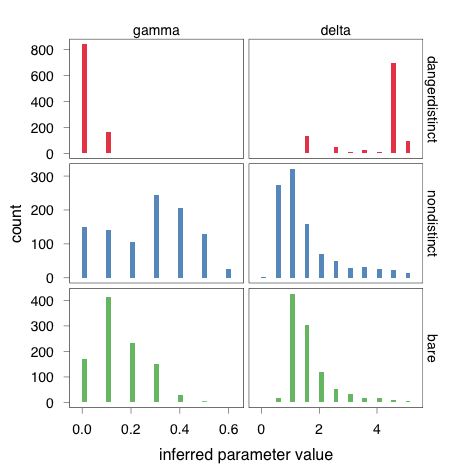
\includegraphics[width=\columnwidth]{fig4_bda2_hyper}
%    \caption{Hyperprior parameters for lifted-variable RSA model}
%  \label{fig:bda2hyperparams}
%\end{figure}

\subsection{Results}

\subsubsection{Inferred parameters}
We use this data analysis model to infer the hyperprior parameter values (\lstinline{gamma} and \lstinline{delta}) for lvRSA. Figure \ref{fig:modeldatapriors} (bottom) shows prior distributions from the posterior mean inferred values of the hyperprior parameters. This makes the prediction that, if this were the correct model of human cognition, the prior distribution of the \emph{dangerous \& distinctive} condition would be heavily skewed towards lower prevalence levels. This makes sense insofar as a distinctive feature is one that is relatively rare. Our intuitions are again confirmed in the inferred distribution of the \emph{nondistinctive} context. A nondistinctive feature is one that is very common. The prior distribution of the \emph{bare} context lies somewhere in between these two extremes: neither distinctive nor nondistinctive.

It should also be noted that the mean inferred value of  \lstinline{phi} is about 0.2, a seemingly reasonable estimation of ``guessing'' probability for participants on Amazon's Mechanical Turk.

\subsubsection{Posterior predictives}
The posterior predictions for the lifted variable RSA model are in Figure \ref{fig:bda1posteriorpred} (right). We can see here that model predicts intermediate endorsement rates for the generic at lower prevalence levels. In a sense, the model has some persistent uncertainty about the true value of the threshold, a feature that people share. We reconstruct the curves of Figure \ref{fig:replication} well; the model--data correlation is $r = 0.97$.



%\begin{figure}
%\centering
%    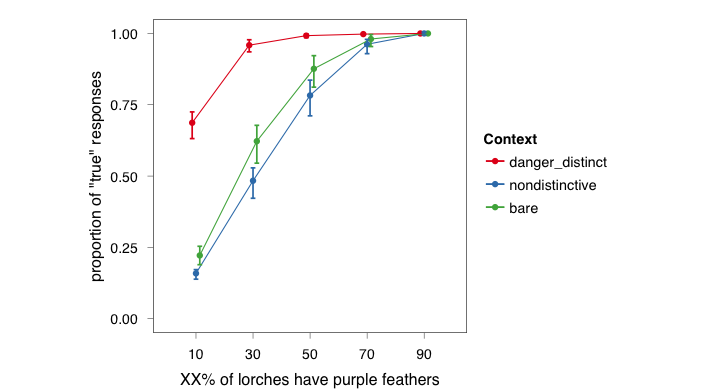
\includegraphics[width=\columnwidth]{fig5_bda2_postpred}
%    \caption{Posterior predictive using lifted-variable RSA}
%  \label{fig:postpred2}
%\end{figure}

In addition to making predictions about the proportion of ``true'' responses to generic statement under different prevalence levels, the combination of the RSA model of language understanding and the bayesian data analysis model gives rise to predictions about the shape of the prior distribution of prevalence levels under different contexts. We take these predictions seriously and test these in a second experiment. 

\section{Experiment 2}

Exp. 2 sought to test the prediction that the prior distribution of prevalence levels would vary by context, as predicted by the $\gamma$ and $\delta$ data analysis parameters from the previous section.

\subsection{Method}

\subsubsection{Participants}

We recruited 30 participants over Amazon's crowd-sourcing platform Mechanical Turk. 

\subsubsection{Procedure and materials}

Our procedure was similar to Exp. 1b\footnote{The experiment in full can be viewed at \url{http://stanford.edu/~mtessler/experiments/generics/cbg2010-replication/experiment/experiment-11.html}}. On each trial, participants either read contextual information (\emph{DD} or \emph{NI}) or nothing (\emph{plain}). 

In addition to thecontextual information, participants were presented with the following: ``Listed below are 5 kinds of animals, recently discovered.'' and asked the following question: ``What percentage of each kind of animal do you think has [property]?'' The experiment consisted of 6 trials, 2 from each context. 

\subsubsection{Results}

Experiment 2 recovered the shape of the inferred prior distributions from the lvRSA model (Figure \ref{fig:modeldatapriors}).

\begin{figure}
\centering
    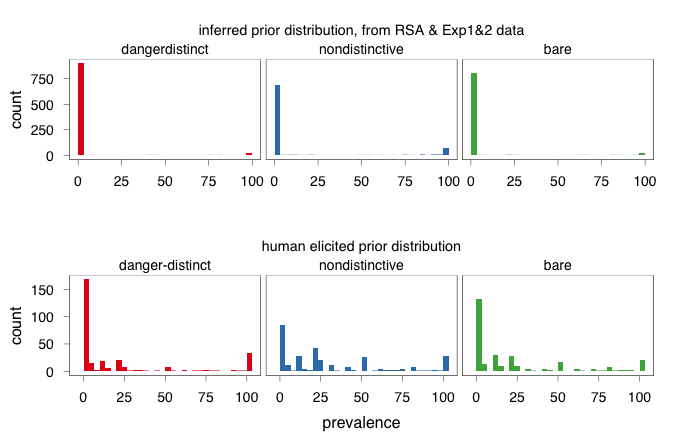
\includegraphics[width=\columnwidth]{exp3hist_inferredMeanPriorExp1_2}
    \caption{Prior distributions over prevalence. Inferred from Bayesian model (top). Elicited from subjects (bottom).}
  \label{fig:modeldatapriors}
\end{figure}


\section{Further simulations}

Our model makes the prediction that if the shape of the prior distribution was not bimodal, the asymmetry between verification and interpretation would change. Indeed, this is a similar prediction to \citeA{Cimpian2010}, who posited that accidental or disease states (e.g. ``muddy feathers'', ``infected ears'') would weaken the asymmetry. We would expect accidental or disease states to not follow a bimodal distribution. 
 

\section{Discussion}

We have shown how a Bayesian model of language understanding, motivated by contextual variation of the effective threshold of the generic statement, can explain the data. We have used technique in Bayesian data analysis to help arbitrate between two cognitive theories. The first was a simple theory that proposed that a generic was akin to some alien quantifier. This quantifier behaves like other quantifiers in that it has a fixed-threshold semantics. The only thing special about the generic is that the threshold is different for different contexts. We believe this is a tacit assumption of many approaches, but that this assumption lay hidden behind NHST of semantic content.

\begin{figure}
\centering
    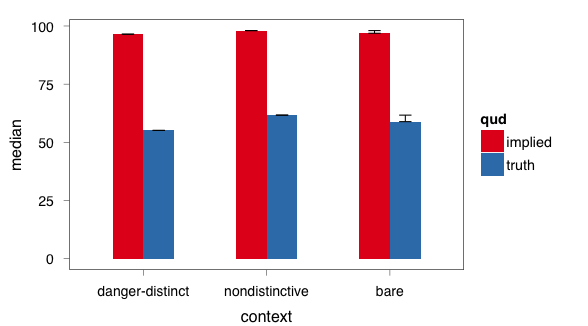
\includegraphics[width=\columnwidth]{asymmetry_byContext_condTwice}
    \caption{Symmetries and asymmetries among dependent measures and quantifiers.}
  \label{fig:asymmetry}
\end{figure}

The alternative theory was that there is no known generic-threshold, even within a given context. There is only uncertainty, and though that uncertainty may be reduced by further contextual information, it never completely evaporates. Instead, we are only left with a posterior belief distribution over possible thresholds as well as a posterior belief distribution over possible worlds. 

In this paper, we used techniques of both Bayesian Cognitive Science and Bayesian Data Analysis. The former helped us develop a rich, formal theory of language understanding. These sorts of theories have implications for psychology and linguistics. The latter helped us make inferences about our theories. Bayesian Data Analysis is crucial to make assumptions explicit (e.g. about fixed-threshold semantics) and clean up our data (e.g. discounting behavior that can conceivably be attributed to guessing). Together, they embody a manifestation of a more general philosophy of science: making assumptions explicit and beginning our science by announcing our uncertainty.

What we're left is an explanation that not all pieces of language need definite semantic content. Mr. Obama's proclamation and the very fact that he went through the trouble to say it suggests that perhaps many members of Congress are able to talk to each other. From another angle, though, 
we can use our knowledge of the world---and the Union---to determine that ``Members of both parties'' supporting Mr. Obama is probably a pretty rare feature; perhaps it would be distinctive of our time (relative to the past). By this logic, the threshold for validly producing the generic could be quite low.  But maybe we shouldn't spend so much energy inferring the threshold, and instead, listen to hear what his other words may suggest.

%\begin{itemize}
%
%\item Replace figure 4 (hyperprior parameters) with mean distribution?
%
%\item Collapse Figure 3 \& 5 (posterior predictive) into one
%
%\item Exp 2 to confirm $\gamma$ and $\delta$. 
%
%\item Some linking function to condition on Exp 1 \& 2 simultaneously,  to perhaps, infer rationality parameter and get some posterior predictives.
%
%\end{itemize}
%
%The data analysis involved comparing the mean of the prevalence ratings associated with \emph{True} endorsements of the generic with the mean prevalence ratings elicited by the generic in a separate task. In the experimental pragmatics literature, the dependent measure involved in the ``truth conditions'' task is called \emph{sentence verification}; in the ``implied prevalence'' task, it is a \emph{sentence interpretation}. 
%
%These different dependent measures, we argue, imply different Questions Under Discussion (QUD, \cite{Roberts2004}). 



%	\section{Sentence verification is a speaker task}
%	
%	DegenGoodman2014.  Truth conditions task --> QUD = ``generic true?'' Model.
%	
%	But what is the semantics of the generic? \citeA{Cimpian2010}, experiments 1, 3, and 4 found that the truth conditions of the generic are sensitive to the context.  Our goal is to replicate this finding, and use Bayesian data analysis to infer the threshold of the speaker model. This bears some similarity to Michael Franke's approach for cogsci from last year.
%	
%	
%	
%	
%	\section{The full bayesian thing}
%	
%	Computational models of cognition typically have parameters. Many of these parameters are of theoretically interest, because they are posited to reside within the head of the subject.
%	
%	\subsection{Inferring quantifier threshold by context}
%	
%	Here we'll find that the generic threshold changes by context. We might also want to show that ``most'' and ``some'' do not change by context.
%	
%	\subsection{Are generics like adjectives?}
%	
%	To determine if a generic is true or false, we must refer to context. The threshold in the threshold-semantic view of the statement varies by context. This property has been shown to be an important feature in the semantics of gradable adjectives (e.g. \emph{tall}) \cite{Lassiter2014}.  
%	
%	\section{Lifted-variable speech act model}
%	
%	We can start in a single context, with a uniform prior over states. We can look at the posterior over states, for listener1. As well, we can look at the posterior over thetas. This depends of course on the alternatives, for which we may want to consider only the experimental alternatives \emph{some, most, generic} or for which we may want to include \emph{all}.  Either way, here we'll recreate the asymmetry between listener and speaker --- between implied prevalence and truth conditions. 
%	
%	\citeA{Cimpian2010} report a ``paradoxical asymmetry at the core of generic meaning'' which manifests as the generic having ``extremely strong implications but requiring little evidence to be judged true''. Here, we explain this ``paradox'' by the different Questions Under Discussions in the tasks used and by the different roles intrinsic to speech-acts: the role of the speaker and the role of the listener. 
%	
%	\subsection{Questions Under Discussion in two tasks}
%	
%	\citeA{Cimpian2010} used two tasks (with different dependent measures) to get at the comparison between ``acceptance'' and ``implications''. These two tasks --- called ``truth conditions'' and ``implied prevalence'' -- used different questions and different dependent measures to get at the meaning of generics. In the ``truth conditions'' task, subjects are given evidence about the prevalence of a property (e.g. ``50\% of morseths have silver fur'') and are asked to judge the corresponding generic (i.e. ``Morseths have silver fur'') to be either true or false. In the ``implied prevalence'' task, subjects are given a generic statement and asked ``What percentage of morseths do you think have silver fur?''
%	
%	\citeA{Degen2014} argue that the \emph{sentence verification} (``truth conditions'') task should be modeled as a speaker task, and that the \emph{sentence interpretation} (``implied prevalence'') task should be modeled as a listener task. In addition to different communicative roles, there are also different implicit Questions Under Discusision. In the ``truth conditions'' task, the QUD seems to be ``is the generic true or false?'', whereas in the ``implied prevalence'' task, the QUD seems to be ``what percentage of category X have property Y?''.





\bibliographystyle{apacite}

\setlength{\bibleftmargin}{.125in}
\setlength{\bibindent}{-\bibleftmargin}

\bibliography{generics}


\end{document}


% after cogsci
% prior elicitation for accidental / disease states
% -- asymmetry weakened

% most / some: better experiments
% -- asymmetry X prior analysis

